%%%%%%%%%%%%%%%%%%%%%%%%%%%%%%%%%%%%%%%%%
% Focus Beamer Presentation
% LaTeX Template
% Version 1.0 (8/8/18)
%
% This template has been downloaded from:
% http://www.LaTeXTemplates.com
%
% Original author:
% Pasquale Africa (https://github.com/elauksap/focus-beamertheme) with modifications by 
% Vel (vel@LaTeXTemplates.com)
%
% Template license:
% GNU GPL v3.0 License
%
% Important note:
% The bibliography/references need to be compiled with bibtex.
%
%%%%%%%%%%%%%%%%%%%%%%%%%%%%%%%%%%%%%%%%%

%----------------------------------------------------------------------------------------
%	PACKAGES AND OTHER DOCUMENT CONFIGURATIONS
%----------------------------------------------------------------------------------------

\documentclass{beamer}

\usetheme{focus} % Use the Focus theme supplied with the template
% Add option [numbering=none] to disable the footer progress bar
% Add option [numbering=fullbar] to show the footer progress bar as always full with a slide count

% Uncomment to enable the ice-blue theme
%\definecolor{main}{RGB}{92, 138, 168}
%\definecolor{background}{RGB}{240, 247, 255}

\setbeamertemplate{itemize item}{$\bullet$}
\setbeamertemplate{itemize subitem}{$\checkmark$}

%------------------------------------------------

\usepackage{booktabs} % Required for better table rules

%----------------------------------------------------------------------------------------
%	 TITLE SLIDE
%----------------------------------------------------------------------------------------

%\title{Election-based Key Management Protocol for IoT}
\title{End-of-study internship}

\subtitle{Group Key Management and IoT Security}

\author{Ramy Chemak}

\titlegraphic{
\includegraphics[scale=0.28]{figures/logo-banner.png}} % Optional title page image, comment this line to remove it

\institute{\textit{INSA Centre Val de Loire} \\  \textit{Heudiasyc UMR CNRS 7253}}

\date{August 31\textsuperscript{st} 2021}

%------------------------------------------------

\begin{document}

%------------------------------------------------

\begin{frame}
	\maketitle % Automatically created using the information in the commands above
\end{frame}

\begin{frame}{Overview}
	\begin{itemize}
		\item \textbf{\textit{Stage 1:}} Election-based Key Management Protocol for IoT
		\begin{enumerate}
			\item Literature Review
			\item Election-based protocol
			\item Future works
		\end{enumerate}
		\vfil
		\item \textbf{\textit{Stage 2:}} IoT Security engineering
		\vfil
		\item \textbf{\textit{Conclusion \& Feedback}}
	\end{itemize}
\end{frame}

\section{Stage 1: \\Election-based Key Management Protocol for IoT}

\begin{frame}{Stage 1}
	\begin{enumerate}
		\item Literature Review
		\begin{enumerate}
			\item Group Key Management
			\item Multi Group Key Management Protocol
			\item Cluster Head schemes
		\end{enumerate}
		\vfil
		\item Election-based protocol
		\begin{enumerate}
			\item Technical Eligibility Criteria
			\item Election process
			\item Failure recovery
			\item Simulation
		\end{enumerate}
		\vfil
		\item Future works
	\end{enumerate}
\end{frame}

\section{Literature Review}

\begin{frame}{Group Key Management: Sum up}
	\begin{itemize}
		\item Network subdivided into several groups
		\item[$\bullet$] Each network node belong to a group
		\item[$\bullet$] The Key Manager (KM) manages different cryptographic keys
		\item Security considerations:
		\begin{itemize}
			\item Forward secrecy
			\item Backward secrecy
			\item Collusion attack recovery
		\end{itemize}
	\end{itemize}
\end{frame}

\begin{frame}{Group Key Management: Problematic}
	The KM is responsible for:
	\begin{itemize}
		\item rekeying the group when needed
		\item generating keys for joining nodes
		\item revoking keys for leaving nodes
	\end{itemize}
	\pause
	\vfill
	\begin{alertblock}{Single point of failure}
		The Key Manager is responsible for the network's security infrastructure. Hence, its breakdown or compromise can jeopardize the overall network's security.
	\end{alertblock}
\end{frame}

\begin{frame}{Multi Group Key Management Protocol}
	\begin{itemize}
		\item Subdivided into 3 layers
		\item Considerate multi services and heterogeneous networks
	\end{itemize}
	\vfill
	\centering
	\begin{figure}
		\centering
		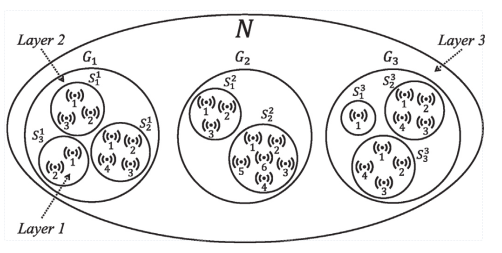
\includegraphics[scale=0.40]{figures/mgkmp/mgkmp_layers.png}\\
		\caption{Source \cite{kandi_versatile_2020}: Example of a network partitioning}
	\end{figure}
\end{frame}

\begin{frame}{MGKMP: Working tracks and proposals}
	\begin{itemize}
		\item Analysis of an n-tier architecture
	\end{itemize}
	\vfill
	\centering
	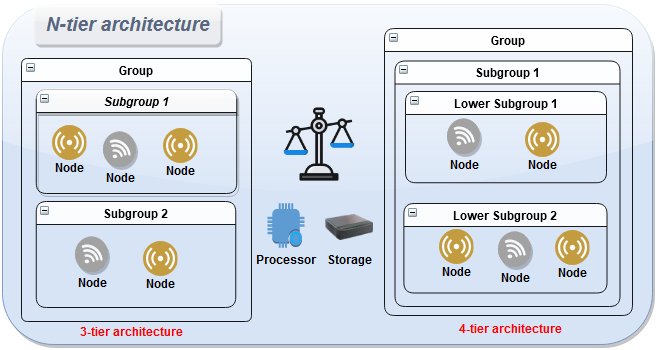
\includegraphics[scale=0.37]{figures/mgkmp/n-tier.png}
\end{frame}

\begin{frame}{MGKMP: Working tracks and proposals}
	\begin{itemize}
		\item Analysis of an n-tier architecture
		\item Re-order algorithm upon leave
	\end{itemize}
	\vfill
	\centering
	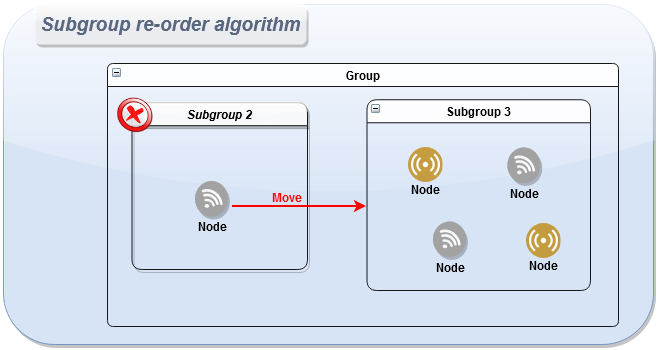
\includegraphics[scale=0.37]{figures/mgkmp/reorder.png}
\end{frame}

\begin{frame}{MGKMP: Working tracks and proposals}
	\begin{itemize}
		\item Analysis of an n-tier architecture
		\item Re-order algorithm upon leave
		\item Sub-grouping sequences
	\end{itemize}
	\vfill
	\centering
	\begin{figure}
		\centering
		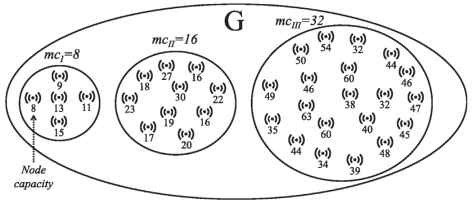
\includegraphics[scale=0.37]{figures/mgkmp/power2.png}\\
		\caption{Source \cite{kandi_versatile_2020}: Example of a group partitioned using powers of 2
sequence}
	\end{figure}
\end{frame}

\begin{frame}{MGKMP: Working tracks and proposals}
	\begin{itemize}
		\item Analysis of an n-tier architecture
		\item Re-order algorithm upon leave
		\item Sub-grouping sequences
		\item Refresh key generation
	\end{itemize}
	\vfill
	\centering
	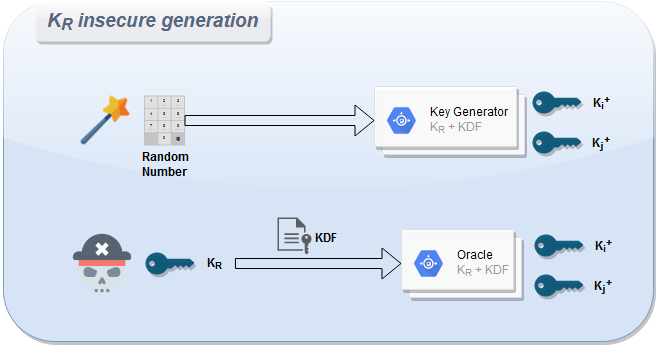
\includegraphics[scale=0.37]{figures/mgkmp/random.png}
\end{frame}

\begin{frame}{MGKMP: Working tracks and proposals}
	\begin{itemize}
		\item Analysis of an n-tier architecture
		\item Re-order algorithm upon leave
		\item Sub-grouping sequences
		\item Refresh key generation
		\item Node’s join authorization \& pre-secure channel
	\end{itemize}
	\vfill
	\centering
	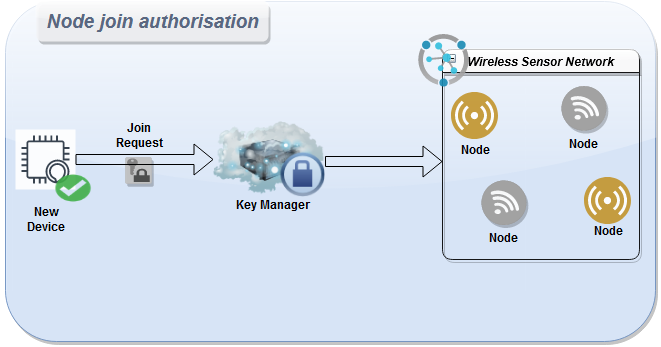
\includegraphics[scale=0.37]{figures/mgkmp/join_auth.png}
\end{frame}

\begin{frame}{MGKMP: Working tracks and proposals}
	\begin{itemize}
		\item Analysis of an n-tier architecture
		\item Re-order algorithm upon leave
		\item Sub-grouping sequences
		\item Refresh key generation
		\item Node’s join authorization \& pre-secure channel
		\item Key Manager's single point of failure
	\end{itemize}
\end{frame}

\begin{frame}{Cluster Head schemes}
	\begin{itemize}
		\item First considered for network routing purposes
		\item Network nodes are grouped in several groups or clusters
		\item Each group has its own Cluster Head, which is no more than one of its nodes
	\end{itemize}
	\vfill
	\centering
	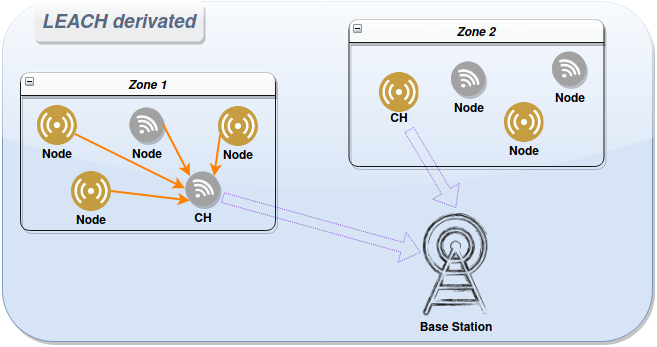
\includegraphics[scale=0.35]{figures/LEACH.png}
\end{frame}

\begin{frame}{Retained proposal}
	\begin{alertblock}{Proposed solution}
		By applying Cluster Head schemes to Group Key Management (GKM), we are able to achieve a decentralized GKM architecture which solves the single point of failure's issue. 
	\end{alertblock}
	\vfill
	\centering
	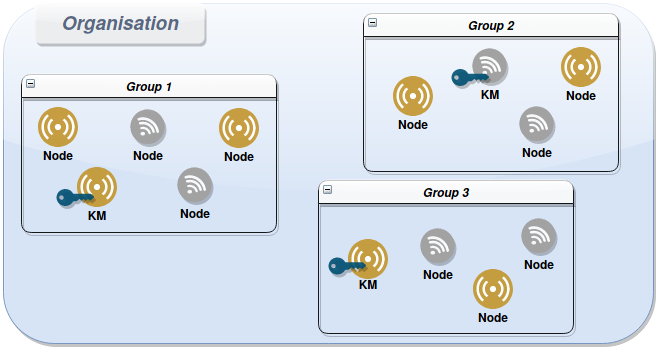
\includegraphics[scale=0.32]{figures/organisation.png}
\end{frame}

\section{Election-based protocol}

\begin{frame}{Workflow overview}
	\begin{itemize}
		\item New decentralized solution for GKM
		\begin{itemize}
			\item Capacity Evaluation Function
			\item Election process
			\item Failure recovery
		\end{itemize}
		\item Simulations
		\item International conference paper
	\end{itemize}
\end{frame}

\begin{frame}{Technical Eligibility Criteria}
	\begin{columns}
		\column{0.5\textwidth}
		\begin{itemize}
			\item Ensure the KM's reliability
			\item Considerate the nodes capacities:
			\begin{itemize}
				\item Storage
				\item Networking
				\item Processing
			\end{itemize}
			\item Also considerate energy
		\end{itemize}
		\column{0.5\textwidth}
		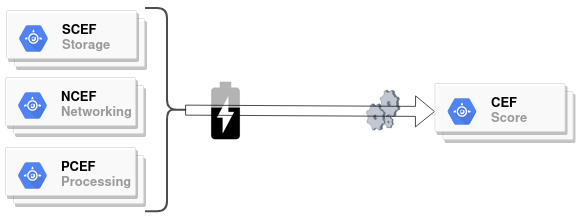
\includegraphics[width=\linewidth]{figures/cef_simple2.png}
	\end{columns}
	%Technical Eligibility Criteria ...
	%\centering
	%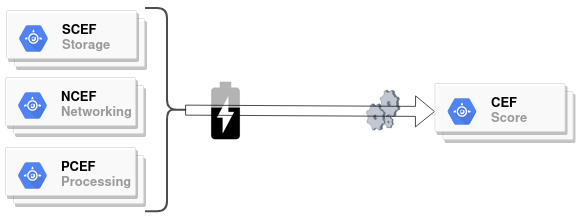
\includegraphics[width=\linewidth]{figures/cef_simple2.png}
\end{frame}

\begin{frame}{Technical Eligibility Criteria}
	\begin{exampleblock}{Capacity Evaluation Function score}
		\begin{equation*}
			c_k = e_k \; .\; \left( w_s s_k + w_n n_k +  w_p p_k \right)
		\end{equation*}
	\end{exampleblock}
	\vfill
	where
	\begin{math}
		\left\{
		\begin{array}{l}
			c_k: capacity\; score\; of\; a\; node\; u_k\\
			e_k: energy\; attribute\; of\; a\; node\; u_k\\
			s_k: storage\; capacity\; of\; a\; node\; u_k\\
			p_k: processing\; capacity\; of\; a\; node\; u_k\\
			n_k: networking\; capacity\; of\; a\; node\; u_k\\
			w_i: capacities\; weights
		\end{array}
		\right.
	\end{math}
\end{frame}

\begin{frame}{Election process}
	\begin{columns}
		\column{0.55\textwidth}
		\begin{itemize}
			\item All nodes are voters, but not all are eligibles candidates
			\item Eligible nodes broadcast their CEF score
			\item Nodes vote for best two candidates
			\item Elected Key Manager \& Deputy KM claim their roles
		\end{itemize}
		\column{0.45\textwidth}
		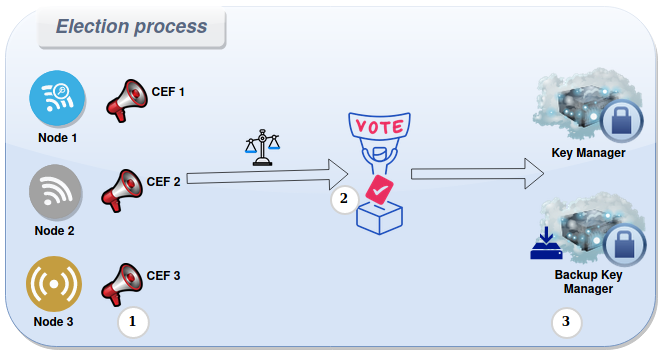
\includegraphics[width=\linewidth]{figures/election.png}
	\end{columns}
\end{frame}

\begin{frame}{Election process}
	%Election process ...\\
	%lalal\\
	\centering
	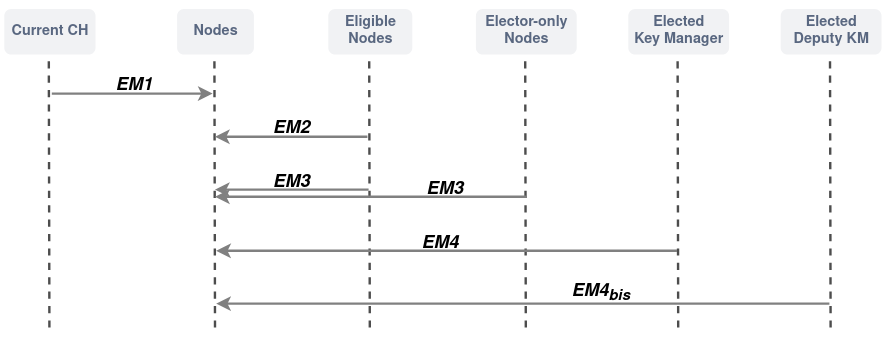
\includegraphics[width=\linewidth]{figures/election_exchange2.png}
\end{frame}

\begin{frame}{Failure recovery}
	\begin{itemize}
		\item Security enforcement
		\item Maintain Integrity \& Availability
	\end{itemize}
	\vfill
	\centering
	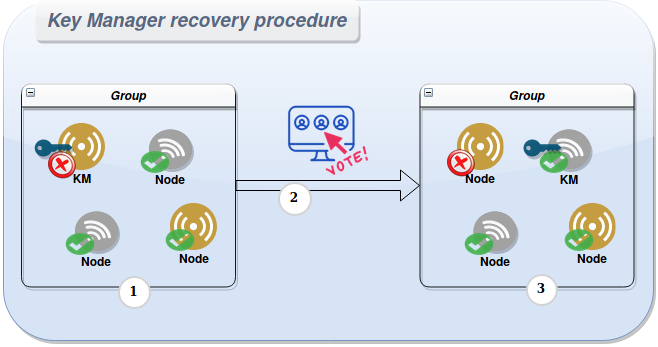
\includegraphics[scale=0.35]{figures/recovery.png}
\end{frame}

\begin{frame}{Failure recovery}
	\begin{columns}
		\column{0.55\textwidth}
		\begin{itemize}
			\item Security enforcement
			\item Maintain Integrity \& Availability
			\item Two check-over routines
			\begin{enumerate}
				\item Simple check-over
				\item Double check-over
			\end{enumerate}
			\item Performance-security compromise
		\end{itemize}
		\column{0.45\textwidth}
		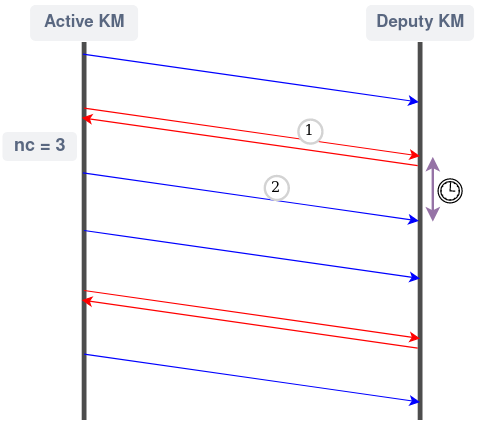
\includegraphics[width=\linewidth]{figures/check_routine_min.png}
	\end{columns}
\end{frame}

\begin{frame}{Failure recovery}
	\begin{columns}
		\column{0.55\textwidth}
		\begin{itemize}
			\item Double check-over
			\item Challenge-response procedure
			\item Requires fast \& correct answer
			\item Ensures both integrity \& availability
		\end{itemize}
		\column{0.45\textwidth}
		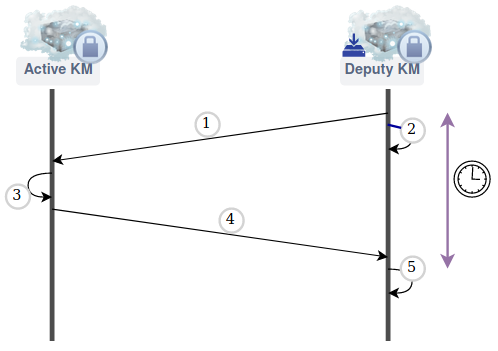
\includegraphics[width=\linewidth]{figures/check_over.png}
	\end{columns}
\end{frame}

\begin{frame}{Simulation}
	\begin{columns}
		\column{0.35\textwidth}
		We are able to quickly reach a satisfactory performance-security compromise.
		\column{0.65\textwidth}
		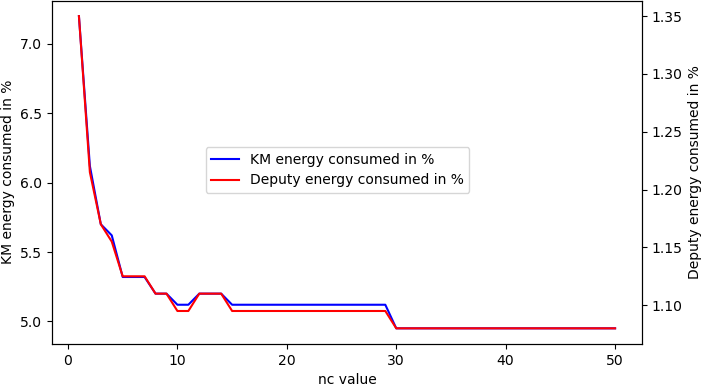
\includegraphics[width=\linewidth]{figures/nc_energy_center2.png}
	\end{columns}
\end{frame}

\begin{frame}{International publication}
	\begin{itemize}
		\item Conference paper in the proceedings of the \emph{\textbf{International Conference on Communications Software (SoftCOM 2021)}}
		\item Acceptance notification received on July 23\textsuperscript{rd} 2021
	\end{itemize}
	\vfil
	\centering
	
\includegraphics[scale=0.20]{figures/SoftCOM-Logo.png}
\end{frame}

\section{Future works}

\begin{frame}{Future works}
	\begin{itemize}
		\item More advanced simulations
		\pause
		\item Real-environment experiments
		\pause
		\item Revision of the current protocol
	\end{itemize}
\end{frame}

\section{Stage 2: IoT Security engineering}

\begin{frame}
	\begin{itemize}
		\item Threats landscape IoT
		\begin{itemize}
			\item IoT Malwares
		\end{itemize}
		\pause
		\vfil
		\item Common IoT vulnerabilities
		\begin{itemize}
			\item Default passwords
			\item Irregular updates
			\item IoT fleet management
			\item $\ldots$ etc
		\end{itemize}
	\end{itemize}
\end{frame}

\section{Conclusion \& Feedback}

\begin{frame}[focus]
	Thanks for your attention !
\end{frame}

\appendix

\begin{frame}{References}
	\nocite{*} % Display all references regardless of if they were cited
	\bibliography{example.bib}
	\bibliographystyle{plain}
\end{frame}

%------------------------------------------------

\begin{frame}{Technical Eligibility Criteria}
	\begin{block}{Storage Capacity Evaluation Function}
		\begin{equation*}
			s_k = pm \; .\; \frac{sc_k}{ks}
		\end{equation*}
	\end{block}
	\vfill
	where
	\begin{math}
		\left\{
		\begin{array}{l}
			s_k: storage\; capacity\; of\; a\; node\; u_k\\
			sc_k: storage\; capability\; of\; a\; node\; u_k\\
			pm: usable\; percentage\; of\; memory\; by\; protocol\\
			ks: size\; of\; a\; key
		\end{array}
		\right.
	\end{math}
\end{frame}

\begin{frame}{Technical Eligibility Criteria}
	\begin{block}{Processing Capacity Evaluation Function}
		\begin{equation*}
			p_k = pp \; .\; \frac{cc_k}{cs \; .\; \left( p + m_j \right)}
		\end{equation*}
	\end{block}
	\vfill
	where
	\begin{math}
		\left\{
		\begin{array}{l}
			p_k: processing\; capacity\; of\; a\; node\; u_k\\
			cc_k: computation\; capability\; of\; a\; nod\;e u_k\\
			pp: usable\; percentage\; of\; processor\; by\; protocol\\
			cs: overhead\; of\; crypto\; system\\
			p: number\; of\; subgroups\; of\; the\; group\; G\\
			m_j: number\; of\; nodes\; in\; subgroup\; S_j
		\end{array}
		\right.
	\end{math}
\end{frame}

\begin{frame}{Technical Eligibility Criteria}
	\begin{block}{Networking Capacity Evaluation Function}
		\begin{equation*}
			n_k = bw_k \; .\; \frac{rr_k}{\left( p + m_j \right) \; .\; \max\left( ms \right)}
		\end{equation*}
	\end{block}
	\vfill
	where
	\begin{math}
		\left\{
		\begin{array}{l}
			n_k: networking\; capacity\; of\; a\; node\; u_k\\
			bw_k: bandwidth\; of\; u_k\; usable\; by\; the\; protocol\\
			rr_k: radio\; range\; of\; u_k\\
			ms: size\; of\; a\; message\\
			p: number\; of\; subgroups\; of\; the\; group\; G\\
			m_j: number\; of\; nodes\; in\; subgroup\; S_j
		\end{array}
		\right.
	\end{math}
\end{frame}

\begin{frame}{Technical Eligibility Criteria}
	\begin{block}{Energy correlation}
		\begin{equation*}
			e_k = \frac{re_k}{ed_k \; .\; pu_k}
		\end{equation*}
	\end{block}
	\vfill
	where
	\begin{math}
		\left\{
		\begin{array}{l}
			e_k: energy\; attribute\; of\; a\; node\; u_k\\
			re_k: residual\; energy\; of\; a\; node\; u_k\\
			ed_k: energy\; drainage\; of\; u_k\\
			pu_k: percentage\; of\; processor\; in\; use\; for\; u_k
		\end{array}
		\right.
	\end{math}
\end{frame}

\begin{frame}{Protocol revision}
	\begin{block}{Energy correlation (plain)}
		\begin{equation*}
			e_k = \frac{re_k}{ed_k \; .\; pu_k}
		\end{equation*}
	\end{block}
	\vfill
	\centering
	OR
	\vfill
	\begin{block}{Energy correlation (configurable)}
		\begin{equation*}
			e_k = \frac{re_k^{\alpha}}{ed_k^{\beta} \; .\; pu_k^{\gamma}}
		\end{equation*}
	\end{block}
\end{frame}

%----------------------------------------------------------------------------------------

\end{document}